
\section{Anhang}

\subsection{Detaillierter Start des Backends auf dem HIMMUC}\label{par:detailed_himmuc}

Um Mandelbrot manuell auf dem Host-System zu installieren,
müssen zunächst die notwendigen Bibliotheken installiert werden.
Eine Anleitung dazu findet sich in \autoref{par:himmuc_install_libs}.
Dies muss nur einmal ausgeführt werden, anschließend können die
Programme wie in \autoref{par:himmuc_build_backend} beschrieben kompiliert werden.
Ist dies nicht gewünscht oder erledigt muss das Backend lediglich noch wie
in \autoref{par:himmuc_run_backend} beschrieben gestartet werden.

\paragraph{Start des Backends}
\begin{figure}[h!]
	\begin{lstlisting}[language=bash, caption={Starten der Entwicklungsumbegung des Backends}]
# Systemabhängige Installation der Docker Anwendung
$ sudo apt install docker
cd backend/ && ./run_docker.sh
Starting the Build Process
...
Host: Core 37 ready!
# ^C beendet das Backend und verbindet sich mit der shell des Containers
^C[mpiexec@9cc2d5ac2cd1] Sending Ctrl-C to processes as requested
[mpiexec@9cc2d5ac2cd1] Press Ctrl-C again to force abort
# exit schliesst die shell des Containers
root@9cc2d5ac2cd1:~/eragp-mandelbrot/backend# exit
        \end{lstlisting}
\end{figure}

\begin{figure}
	\begin{lstlisting}[language=bash, caption={Beispielausgabe bei Start der Entwicklungsumbegung auf dem HimMUC}, label={shell:start_himmuc_example}]
$ eragp-mandelbrot/backend$ python3 himmuc/start_himmuc.py muendler 10 9
Uploading backend...  sending incremental file list
backend/himmuc/start_backend.py
          3,897 100%    3.05MB/s    0:00:00 (xfr#1, to-chk=35/62)
done
Start mandelbrot with 1 host and 9 workers on 9 nodes... started mandelbrot
Search host node... srun: error: Could not find executable worker
odr00 found
Establish port 9002 forwarding to host node odr00:9002 ... established
System running. Websocket connection to backend is now available at
        ws://himmuc.caps.in.tum.de:9002
Press enter (in doubt, twice) to stop Warning: Permanently added the ED25519 host key for IP address '10.42.0.54' to the list of known hosts.
# Enter

Stopping port forwarding... stopped (-9)
Stopping mandelbrot host and workers... stopped (-9)
    \end{lstlisting}
\end{figure}

\paragraph{Lokale Installation der Bibliotheken}\label{par:himmuc_install_libs}


Da hierbei davon ausgegangen wird, dass keine root-Rechte auf dem
Server existieren, werden die Bibliotheken hier lokal in \verb|~/.eragp-mandelbrot|
installiert.
Achten Sie darauf, dass sie Schreibrechte auf dem Ordner haben und
falls sie einen anderen Ordner verwenden wollen,
ersetzen sie jedes Vorkommen des Pfades durch ihren Pfad (insbesondere in der Datei \verb|CMakeLists.txt|).
Die MPI-Bibliothek ist auf dem HimMUC Cluster bereits vorinstalliert
und muss daher nicht mehr aufgesetzt werden.
\begin{figure}[h!]
	\begin{lstlisting}[language=bash, caption={Erstellen des Installationsordners}]
mkdir ~/.eragp-mandelbrot
    \end{lstlisting}
\end{figure}

Die 'Header-only' Libraries \verb|websocketpp| und \verb|rapidjson| müssen
lediglich an einen fixen Ort kopiert werden.
Dies erledigen die Befehle aus \autoref{shell:install_header_libs}.

\begin{figure}[h!]
	\begin{lstlisting}[language=bash, caption={Lokale Installation der Bibliotheken \texttt{websocketpp} und \texttt{rapidjson}.}, label={shell:install_header_libs}]
mkdir "~/.eragp-mandelbrot/install"
cd "~/.eragp-mandelbrot/install"
# Installation von websocketpp
git clone --branch 0.7.0 https://github.com/zaphoyd/websocketpp.git websocketpp --depth 1
# Installation von rapidjson
git clone https://github.com/Tencent/rapidjson/
    \end{lstlisting}
\end{figure}


Aus der Bibliothek \verb|boost| muss die Teilbibliothek \verb|boost_system| lokal kompiliert werden
Dazu werden die Befehle aus \autoref{shell:install_boost} ausgeführt,
um die Version 1.67.0 herunterzuladen, zu entpacken und lokal zu installieren.
Beachten Sie, dass das kompilieren auch wie in \autoref{par:himmuc_build_backend} beschrieben
von einem der Boards ausgeführt werden muss.

\begin{figure}[h!]
    \begin{lstlisting}[language=bash, caption={Lokale Installation der Bibliothek boost.}, label={shell:install_boost}]
# Erstellen der notwendigen Ordnerstrukturen
mkdir "~/.eragp-mandelbrot/install"
mkdir "~/.eragp-mandelbrot/local"
# Einrichten des Internetproxys
export http_proxy=proxy.in.tum.de:8080
export https_proxy=proxy.in.tum.de:8080
# Herunterladen und kompilieren der Boost-Bibliothek
cd "~/.eragp-mandelbrot/install"
wget "https://dl.bintray.com/boostorg/release/1.67.0/source/boost_1_67_0.tar.bz2"
tar --bzip2 -xf boost_1_67_0.tar.bz2
cd boost_1_67_0
./bootstrap.sh --prefix="$HOME/.eragp-mandelbrot/local/" --with-libraries=system
./b2 install
    \end{lstlisting}
\end{figure}

\paragraph{Kompilieren des Backends}\label{par:himmuc_build_backend}

Stellen Sie zunächst sicher, dass auf dem Cluster die Quelldateien des Backendes (im Ordner \verb|backend/|) liegen
(zum Beispiel über \verb|rsync| oder indem sie das Repository dort auch klonen)
Zum Kompilieren des Backends sollte sich auf einen Raspberry Pi oder ODroid
per ssh eingeloggt werden\footnote{Es existiert ein Entwicklerzugang zu einem geteilten Raspberry Pi über die Adresse \url{sshgate-gepasp.in.tum.de}. Dieser wird auch vom Pythonskript genutzt}

Auf dem Board, aus dem Ordner des Backendquellcodes müssen Sie zum kompilieren
des Backendes die Befehle aus \autoref{shell:himmuc_compile_backend} ausführen.

\begin{figure}[h!]
	\begin{lstlisting}[language=bash, caption={Kompilieren des Backends}, label={shell:himmuc_compile_backend}]
# Erstellen und betreten eines build Ordners
mkdir build
cd build
# Aktivieren der MPI Bibliothek
module load mpi
# Kompilieren
cmake ..
make
    \end{lstlisting}
\end{figure}


\paragraph{Ausführen des Backends}\label{par:himmuc_run_backend}

Um das Backend auf dem HimMUC Cluster laufen zu lassen, muss sich zunächst darauf per ssh eingeloggt werden.
Damit für das Frontend kein Unterschied dazwischen besteht, ob das Backend im Dockercontainer , oder
auf einem externen Server ausgeführt wird, ist bei der ssh-Verbindung der Port 9002
des \verb|himmuc.caps.in.tum.de|-Servers an den lokalen Port 9002 gebunden.
So ist das Backend stets unter \url{localhost:9002} verfügbar.
Der zugehörige Befehl zum Login lautet demnach:

\begin{lstlisting}[language=bash]
ssh <rechnerkennung>@himmuc.caps.in.tum.de -L localhost:9002:localhost:9002
\end{lstlisting}

Anschließend muss aus dem Ordner, in dem die ausführbaren Dateien liegen,
für gewöhnlich also der \verb|~/.eragp-mandelbrot/build/| Ordner,
folgender Befehl ausgeführt werden:

\begin{lstlisting}[language=bash]
srun -p <odr|rpi> -n <number of workers+1> -N <number of nodes/raspis> -l --multi-prog <path to eragp-mandelbrot/backend>/himmuc/run.conf &
ssh -L 0.0.0.0:9002:localhost:9002 -fN -M -S .tunnel.ssh <odr|rpi><host number>
\end{lstlisting}

Dabei bestimmt \verb|-n| die Anzahl der laufenden Prozesse (Also Hostprozess und Workerprozesse)
und \verb|-N| die Anzahl zu verwendender Rechenknoten.
Damit anschließend noch alle Anfragen an den Websocketserver auf dem Hostknoten weitergeleitet werden,
muss noch der Port 9002 des \url{himmuc.in.caps.tum.de}-Servers an den Port 9002 des Rechenknotens gebunden werden,
auf dem der Hostprozess läuft.
Der korrekte Knoten ist dabei der Ausgabe des \verb|srun|-Befehles zu entnehmen.
Eine beispielhafte Ausgabe ist in \autoref{shell:himmuc_running_backend_example} zu sehen.

\begin{figure}[h]
	\begin{lstlisting}[language=bash, caption={Beispielhafter Start des Backends. Hierbei ist der Knoten des Hostprozesses \texttt{rpi03}.}, label={shell:himmuc_running_backend_example}]
muendler@vmschulz8:~/eragp-mandelbrot/backend/build$ srun -N4 -n5 -l --multi-prog ../himmuc/run.conf
srun: error: Could not find executable worker
4: Worker: 4 of 5 on node rpi06
2: Worker: 2 of 5 on node rpi04
3: Worker: 3 of 5 on node rpi05
0: Host: 0 of 5 on node rpi03
0: Host init 5
1: Worker: 1 of 5 on node rpi03
0: Core 1 ready!
1: Worker 1 is ready to receive Data.
2: Worker 2 is ready to receive Data.
0: Listening for connections on to websocket server on 9002
0: Core 2 ready!
3: Worker 3 is ready to receive Data.
0: Core 3 ready!
4: Worker 4 is ready to receive Data.
0: Core 4 ready!
muendler@vmschulz8:~/eragp-mandelbrot/backend/build$ ssh ssh -L 0.0.0.0:9002:localhost:9002 -fN -M -S .tunnel.ssh rpi03
    \end{lstlisting}
\end{figure}

\paragraph{Stoppen des Backends}

Um das Backend wieder zu stoppen, müssen der ssh-Tunnel zur Verbindung der Ports
und der \verb|srun|-Prozess gestoppt werden.
Letzterer lässt sich nach dem dämonisieren im vorigen Aufruf nur über die Prozess-ID finden.
Diese zeigt das Tool \verb|ps| an.
\begin{lstlisting}[language=bash]
ssh -S .tunnel.ssh -O exit rpi<host number>
# To stop the node allocation
scancel -u <user name>
\end{lstlisting}

\subsection{Abängigkeiten des Frontends}
\begin{figure}[h!]
	\begin{lstlisting}[language=bash, caption={Starten des Frontends mit beispielhafter Ausgabe}]
# Systemabhängige Installation der npm Paketverwaltung
sudo apt install npm
# Installiert benötigte Bibliotheken und startet WebServer
cd frontend/ && npm install ; npm start
...
Version: webpack 4.25.1
Time: 7230ms
Built at: 12/28/2018 10:48:32 PM
        Asset      Size  Chunks             Chunk Names
   index.html  1.65 KiB          [emitted]
mandelbrot.js  11.7 MiB    main  [emitted]  main
    style.css   519 KiB    main  [emitted]  main
Entrypoint main = style.css mandelbrot.js
...
        \end{lstlisting}
\end{figure}
\begin{figure}[h!]
	\lstinputlisting[caption={Abh\"angigkeiten des Frontends. Verwaltet durch NPM}]{./code/frontend_dependencies.json}
\end{figure}

\subsection{Detaillierte Beschreibung der Header und der CMake Instruktionen}

Die zusammenstellung der ausführbaren Dateien wird in CMake definiert.
Dabei unterscheiden sich diese lediglich in den eingebundenen Quelldateien:
In die Datei \verb|host| werden \verb|host.main.cpp| und \verb|actors/Host.cpp| eingebunden, während
in \verb|worker| \verb|worker.main.cpp| und \verb|actors/Worker.cpp| eingebunden werden.

Diese und alle weiteren Build-Vorgaben werden in der Datei \verb|CMakeLists.txt| für
\verb|cmake|\footnote{Ein Programm, welches die Erstellung von Makefiles vereinfacht in dem es sie automatisch an die Umgebung des Build-Systems anpasst. \url{https://cmake.org/}}
in der hier beschriebenen Reihenfolge spezifiziert.
Es sollte hierbei eine CMake-Version über 3.7.0 gewählt werden und die C++11 Standards\footnote{\url{https://isocpp.org/wiki/faq/cpp11}} werden vorrausgesetzt.
Zudem werden für das Projekt "Mandelbrot" werden alle Dateien im Order \verb|include| eingebunden.
In diesem Ordner liegen die Header-Dateien für alle projektinternen C++-Quelldateien.
Anschließend werden alle C++-Quelldateien (Endung "\verb|.cpp|") aus dem Ordner \verb|src| in einer Liste gesammelt, mit Ausnahme jedoch der oben genannten, exklusiven Quelldateien.
Die erzeugte Liste und die jeweils exklusiven Dateien werden dann den ausführbaren Dateien \verb|host| und \verb|worker| zugeordnet.

Um die verwendeten Bibliotheken verfügbar zu machen werden anschließend die Header der installierten MPI-Bibliothek
sowie die Header der Bibliotheken rapidjson\footnote{\url{http://rapidjson.org}}, websocketpp\footnote{\url{https://github.com/zaphoyd/websocketpp}} und boost\footnote{\url{https://www.boost.org/}}
Diese werden respektive verwendet um JSON zu parsen und enkodieren, Websocket-Verbindungen aufzubauen und darüber zu kommunizieren sowie um diese Bibliothek zu unterstützen.
Da für die boost Bibliothek dabei Header nicht genügen und die systemweite Verfügbarkeit der kompilierten boost-Bibliothek nicht garantiert werden kann, wird die Teilbibliothek boost\_system statisch
in die ausführbaren Datei \verb|host| eingebunden.

Zuletzt werden über Compilerflags alle Kompilierfehler und -warnungen aktiviert sowie die POSIX-Thread-Bibliothek eingebunden,
die Optimierung auf die höchste Stufe gesetzt und spezielle Flags für die Websocketlibrary und MPI gesetzt.

\subsection{Beispielhafte Einbindung der MPI-Initialisierungsfunktion}

Ein beispielhafter Aufruf der Prozessinitialisierung von einer Mainfunktion aus ist in \autoref{src:host.main.cpp} zu sehen. Damit wird MPI initialisiert und nach der
erfolgreichen Initialisierung der eigentliche \hyperref[cls:Host]{Host-Prozess} über \verb|Host::init| gestartet.

\begin{figure}[h]
	\lstinputlisting[caption={Initialisierung des Host-Prozesses in host.main.cpp}, label={src:host.main.cpp}]{../../backend/src/host.main.cpp}
\end{figure}

\begin{figure}
	\lstinputlisting[caption={Initialisierung der MPI-Prozesse in init.cpp}, label={src:init.cpp}, firstline=15, lastline=39, firstnumber=15]{../../backend/src/init.cpp}
\end{figure}

\subsection{Sequenzdiagramm zur Kommunikation im Backend mit Abbruch eines Workers}

Ein Sequenzdiagramm zur Kommunikation im Backend mit Abbruch eines Workers ist in \autoref{fig:mpi_sequenzdiagramm_abbruch} zu finden.

\begin{figure}[ph!]
	% Bindet das als PDF exportierte vsdx ein -> vektorgrafik
	% -> vsdx bearbeiten statt pdf
	\hspace{10mm}
	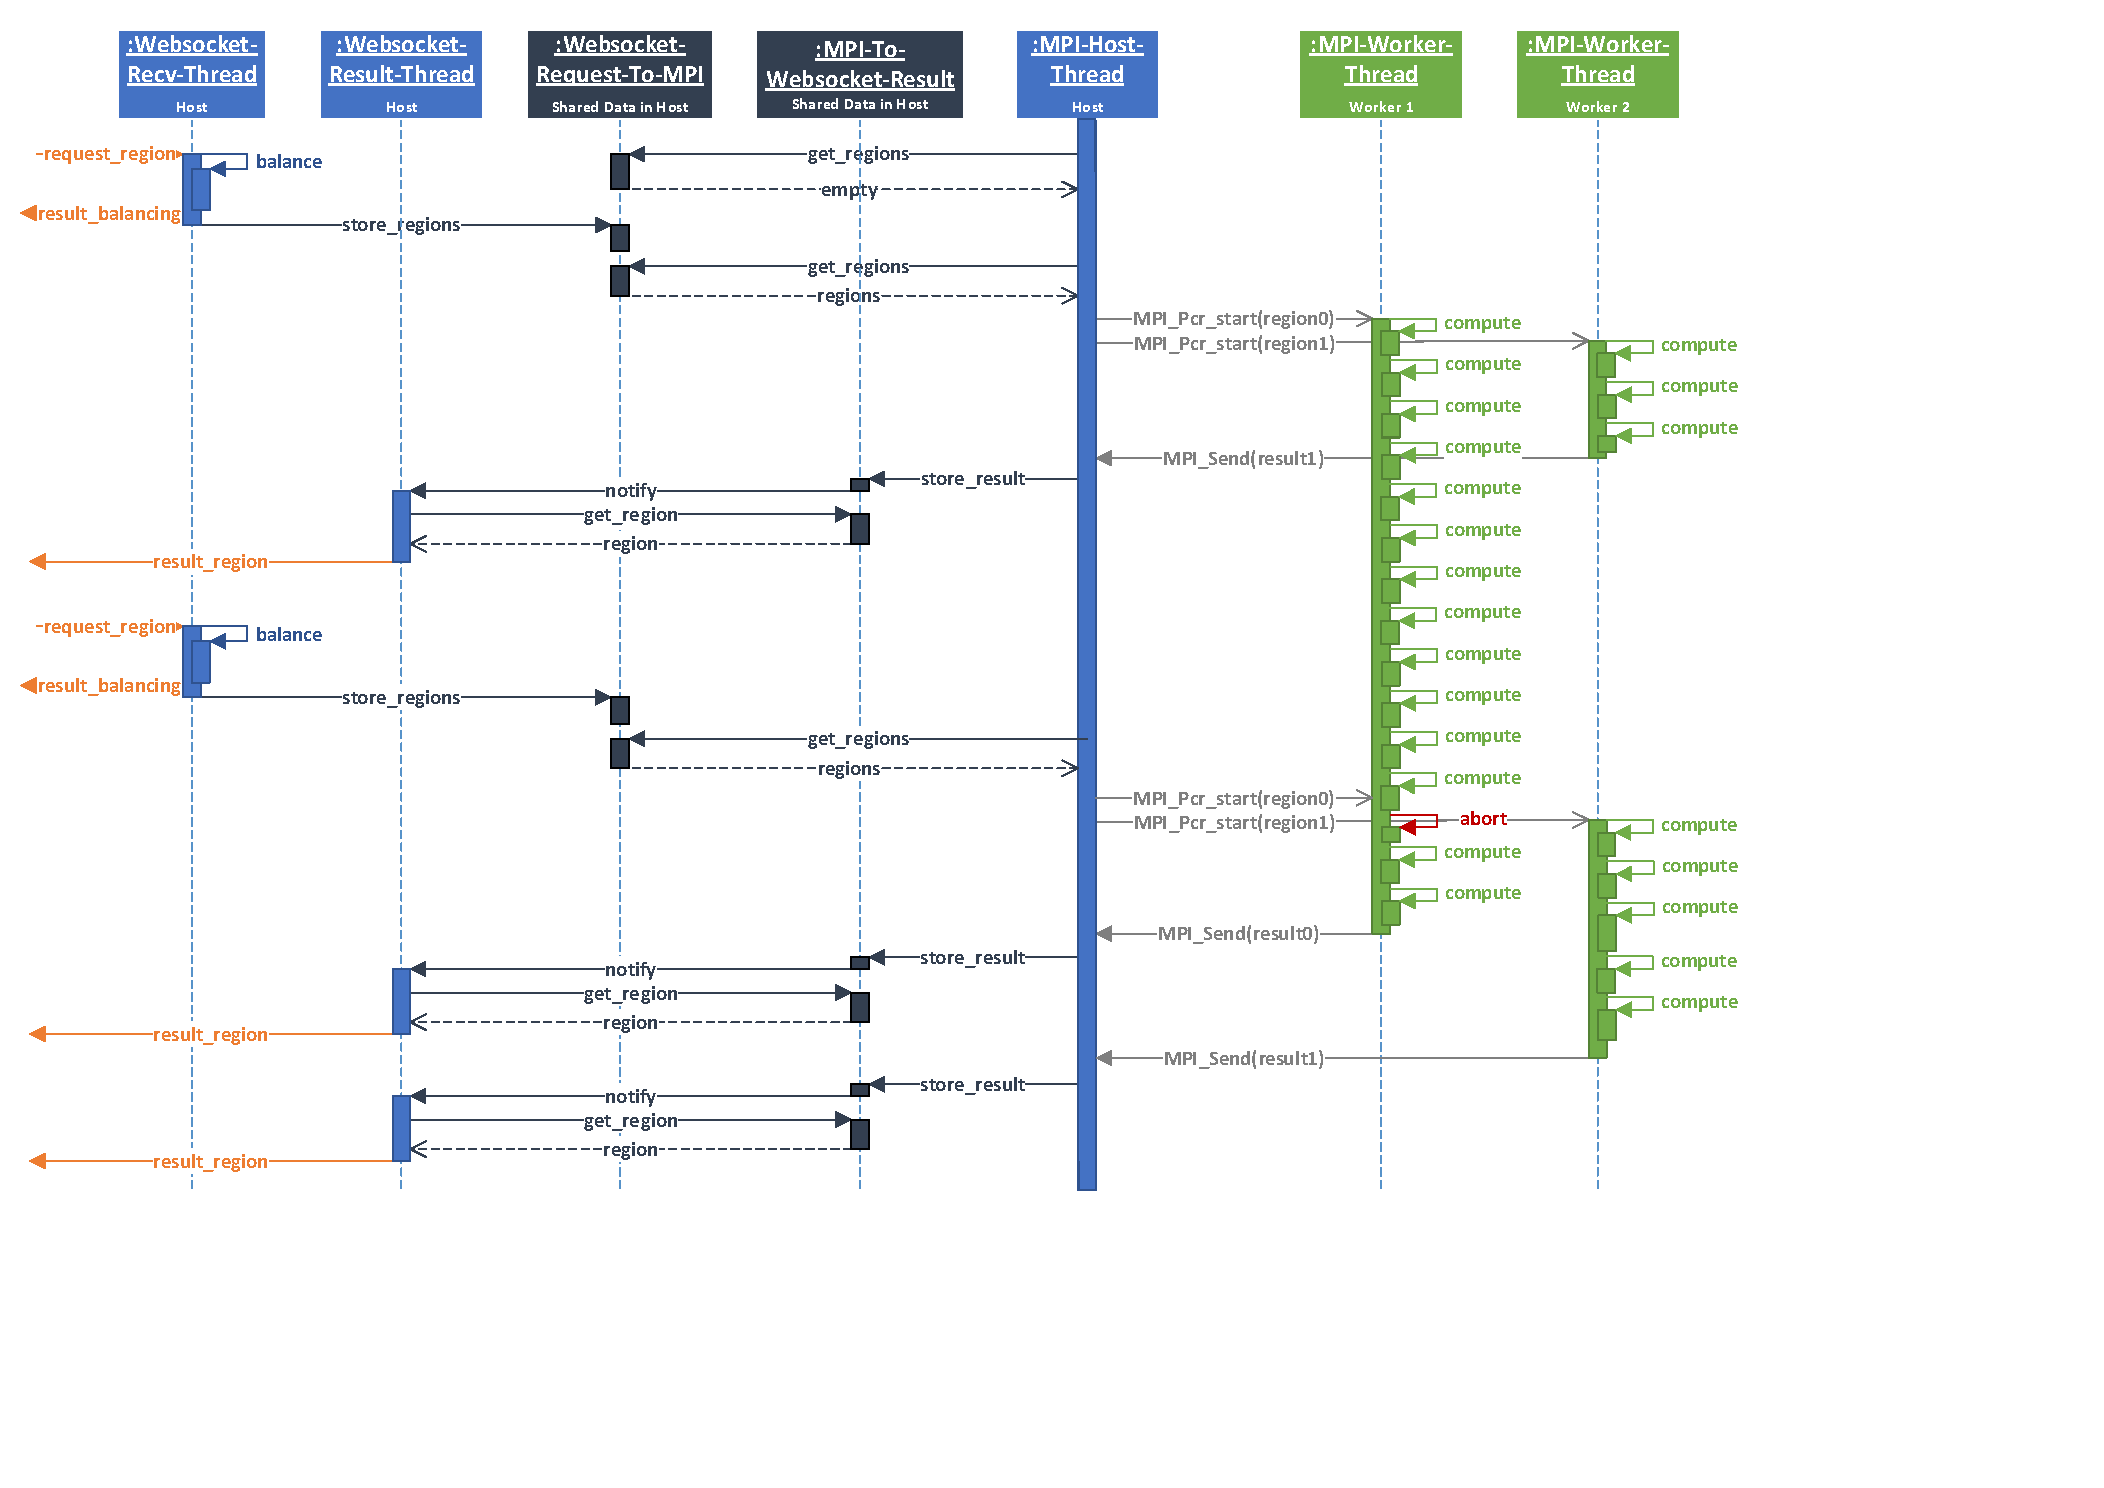
\includegraphics[angle = 90, origin = c, trim = 0mm 0mm 60mm 0mm, clip, width=0.98\linewidth]{img/Implementierung/MPISequenzdiagrammAbbruchFarben.pdf}
	\caption{Sequenzdiagramm zur Kommunikation im Backend mit Abbruch eines Workers}
	\label{fig:mpi_sequenzdiagramm_abbruch}
\end{figure}

\subsection{Detaillierter Ablauf der Host::handle\_region\_request Methode}

Nach dem Parsen der Nachricht wird die Region global festgelegt und beim korrekten Lastbalancierer eine Zerlegung der angefragten Region über \verb|Balancer::balanceLoad| gestartet.

Jeder Region wird ein Worker zugewiesen.
Dabei ist der Rang des Workers, der eine Region berechnen soll genau der Index der Region in dem zurückgegebenen Array.
Ist ein Worker nicht verfügbar, so werden sein und alle folgenden Ränge um eins erhöht (siehe \autoref{src:Host.cpp.handle_region_request}).
Damit kann der Websocketprozess unabhängig von der tatsächlichen Verteilung den Rang des berechnenden Worker-Prozesses
bestimmen und in der Antwort an den Client zu der Aufteilung der Prozesse einfügen.
Die Struktur und eine gültige Antwort des Websocketservers kann \autoref{src:region.json} entnommen werden.

Nachdem die Aufteilung als Antwort auf die Anfrage dem Websocketprozess bereitgestellt wurde, werden die Teilregionen in eine per Mutexlock-gesicherte Datenstruktur
gelegt. Der MPI verwendende Thread, der diese Regionen anschließend an die Worker sendet wird über das Setzen des booleschen Wertes \verb|mpi_set_regions|
auf \verb|true| darüber informiert, dass neue Regionen zum versenden zur Verfügung stehen.

Indem die Regionaufteilung zuerst an das Frontend und anschließend an die Worker gesendet wird,
wird sichergestellt, dass das Frontend alle empfangenen Regionsdaten korrekt der angefragten Region zuordnen kann.
Dabei wird zwar Rechenzeit verschenkt, jedoch steigt durch die Erstellung sehr kleiner oder leerer Teilregionen
die Wahrscheinlichkeit, dass ein Arbeiter mit seiner Region zu früh abgeschlossen ist.
Würde dann dessen Region vor der Gesamtaufteilung beim Frontend ankommen, besteht die Gefahr,
dass es die Daten verwirft.

\begin{figure}
	\lstinputlisting[caption={Algorithmus zur Zuordnung von Regionen auf Worker in Host.cpp}, label={src:Host.cpp.handle_region_request}, firstline=222, firstnumber=222, lastline=231]{../../backend/src/actors/Host.cpp}
\end{figure}

\begin{figure}
	\lstinputlisting[caption={Ausschnitt aus einer gültigen Antwort auf die Region aus \autoref{src:regionRequest.json} in JSON}, label={src:region.json}, language=json]{./code/region.json}
\end{figure}

\subsection{Beispiele für versendete Daten}

\begin{figure}[!h]
	\lstinputlisting[caption={Ausschnitt aus den Daten einer versendeten Teilregion. Punkt (x,y) liegt in \texttt{"data"} an Index $i=x+y*width$.}, label={src:regionData.json}, language=json]{./code/regionData.short.json}
\end{figure}

\subsection{Nutzbarkeit einzelner Worker}

Es besteht die Möglichkeit, explizit zu definieren ob ein Worker Rechenaufträge bekommen soll oder nicht.
Hierzu existiert im Host das globale Boolean-Array usable\_nodes.
Ein Prozess mit Rang x ist benutzbar, wenn usable\_nodes am Index x true ist.
Nicht benutzbar ist er, wenn die Variable auf false gesetzt ist.
Zudem existiert noch die globale Variable usable\_nodes\_count, die angibt wie viele Worker benutzbar sind.
Genutzt wird dieses Feature, falls beim \hyperref[para:init_worker_test]{Initialen Test aller Worker} Worker als nicht benutzbar eingestuft werden.
%TODO: Eventuell noch anmerken, dass man in einer zukünftigen Version herausfinden könnte, ob Worker nach ihrem initialen Test absturzen. Dann kann man sie gleich auf diese Weise ausschalten.

\paragraph{Initialer Test aller Worker}\label{para:init_worker_test}

Bevor Rechenaufträge an die Worker weitergeleitet werden, wird zunächst jeder Worker einzeln getestet.
Dies dient auch dazu, den Workern den Rang des Hosts zu übermitteln.

Dazu sendet der Host mittels der nicht-blockierenden, synchronen Sendeoperation MPI\_Issend einen Test-Wert an alle Worker.
Durch die synchrone Eigenschaft wird die Operation erst abgeschlossen, wenn eine passende Empfangsoperation gestartet und der Sendeoperation zugeordnet wurde.
Es wurde eine nicht-blockierende Sendeoperation gewählt, um den Test für alle Worker parallel ausführen zu können.

Wurden alle Sendeoperationen gestartet, muss auf deren Abschluss gewartet werden.
Falls nun ein Worker nicht wie erwartet reagiert und die Empfangsoperation nicht durchführt, muss das Warten auf den Abschluss der Sendeoperation abgebrochen werden können.
Deshalb wird MPI\_Testsome in einer Endlosschleife genutzt, die nur abbricht falls alle Sendeoperationen erfolgreich waren (alle MPI\_Requests sind MPI\_REQUEST\_NULL, wodurch MPI\_Testsome in outcount MPI\_UNDEFINED zurückgibt) oder ein Timer abgelaufen ist.
Falls eine oder mehrere Sendeoperationen innerhalb eines Schleifendurchlaufs erfolgreich abgeschlossen wurden, wird deren MPI\_Request auf MPI\_REQUEST\_NULL gesetzt um dies explizit zu zeigen.
Sie werden in den nächsten Schleifendurchläufen von MPI\_Testsome ignoriert.

Nachdem die Schleife abgebrochen wurde, muss noch überprüft werden, welche Sendeoperationen erfolgreich waren und welche nicht.
War die Operation erfolgreich, wird der entsprechende Worker als nutzbar eingestuft.
Falls nicht, wird die noch laufende Sendeoperation mit MPI\_Cancel abgebrochen und der Worker als nicht benutzbar eingestuft.

\subsection{Entwicklung des Beschleunigungsfaktors von SIMD für höhere Iterationszahlen}
\label{par:SIMD-speedup-entwicklung}

Wie durch den konstanten Mehraufwand der SIMD-Verwendung zu erwarten, steigt der Beschleunigungsfaktor
monoton und wächst ab circa 6000 Iterationen pro Pixel nicht mehr wesentlich.
Dies kann \autoref{fig:SIMD-speedup-vs-comptime-10000} entnommen werden.

\begin{figure}
	\centering
	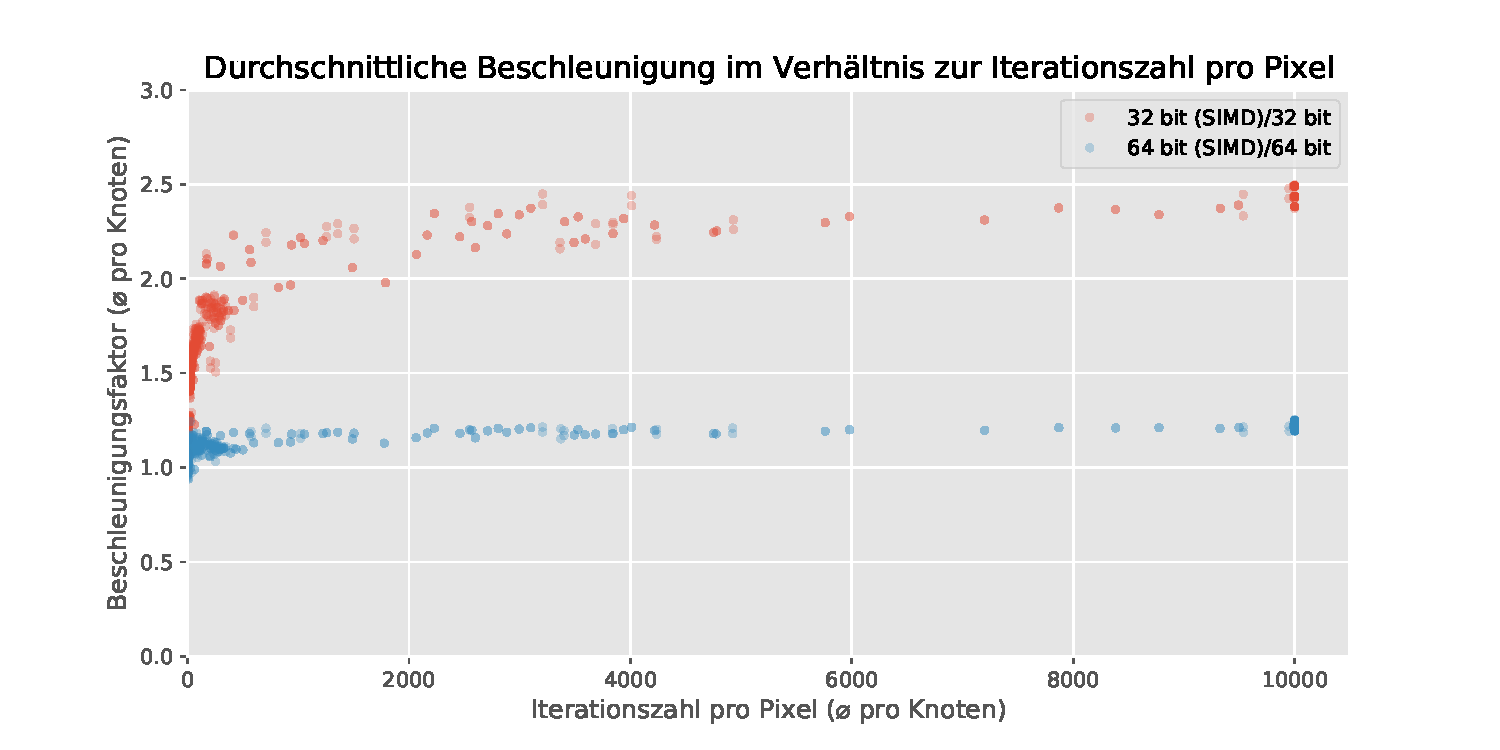
\includegraphics[width=0.9\linewidth]{img/Evaluation/simd/speedup10000.pdf}
	\caption{Beschleunigungsfaktor durch SIMD in Abhängigkeit von der durchschnittlichen Iterationszahl. Auswertung von 360 Regionen mit zwei Durchläufen. Die Iterationszahl für einen Abbruch war 10000.}
	\label{fig:SIMD-speedup-vs-comptime-10000}
\end{figure}

Dass hier auch nicht in der Homogeninät der Iterationszahlen in Bereichen hoher Rechenintensität liegt,
zeigt \autoref{fig:SIMD-speedup-vs-comptime-150}.
Sie hat jedoch einen deutlich erkennbaren Einfluss auf die Beschleunigung.
Während in bei einem frühzeitigen Abbruch bei \hyperref[fig:SIMD-speedup-vs-comptime]{1019 Iterationen} eine Beschleunigung von über 2
erst ab etwa 200 Iterationen gemessen wird, tritt sie bei \hyperref[fig:SIMD-speedup-vs-comptime-150]{maximal 150 Iterationen} bereits ab etwa 140 auf.

\begin{figure}
	\centering
	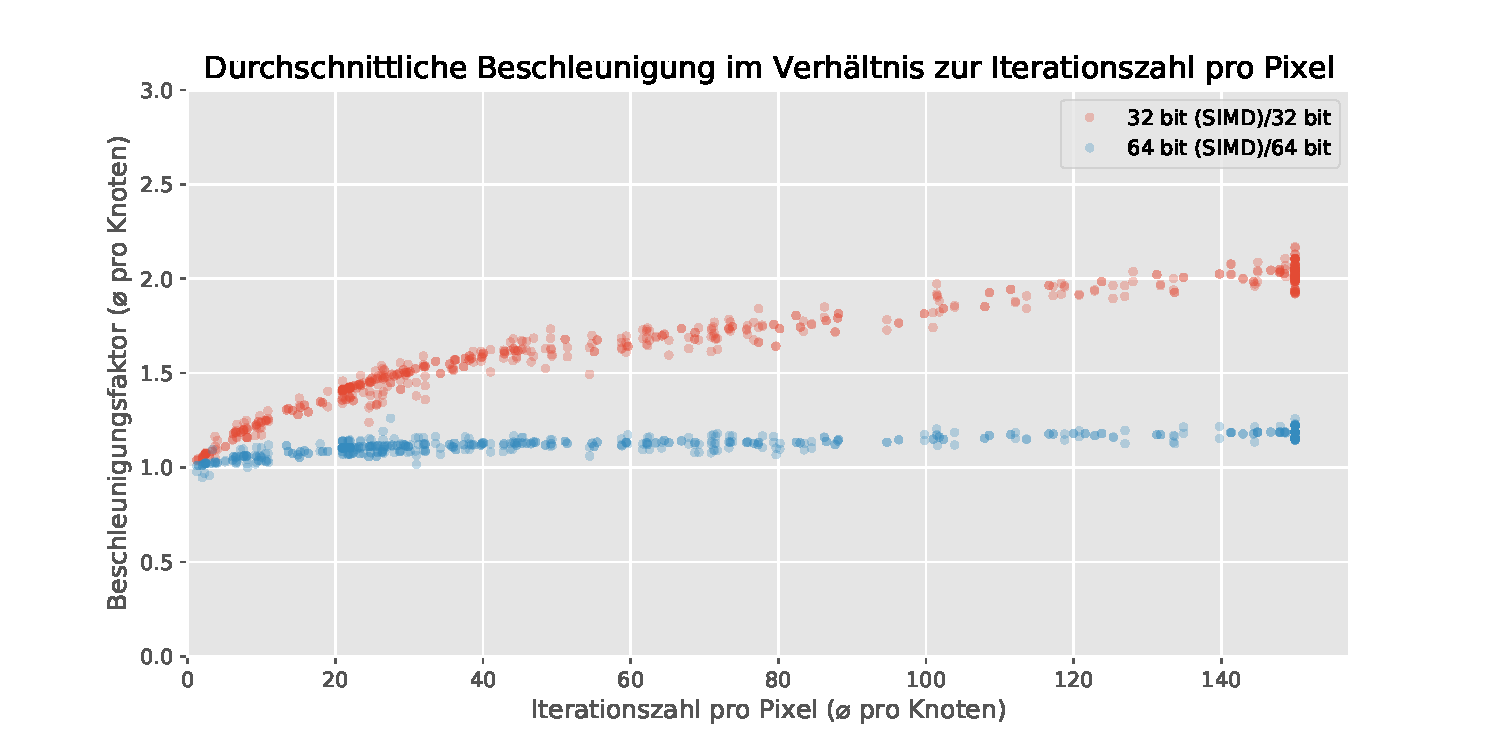
\includegraphics[width=0.9\linewidth]{img/Evaluation/simd/speedup150.pdf}
	\caption{Beschleunigungsfaktor durch SIMD in Abhängigkeit von der durchschnittlichen Iterationszahl. Auswertung von 360 Regionen mit zwei Durchläufen. Die Iterationszahl für einen Abbruch war 150.}
	\label{fig:SIMD-speedup-vs-comptime-150}
\end{figure}

%TODO Eigentlich alles löschen. Ist aktuell nur zur Sicherheit hier, sodass man schnell etwas rauskopieren könnte.
\subsection{Kommunikation der Prozesse per MPI}\label{sec:mpi}

% TODO: Irgendwo muss noch erwähnt werden, dass es nur auf gleichen Rechnern funktioniert, da wir Byte-Ströme übertragen

Das Message Passing Interface (MPI) wird ausschließlich im Backend zur Kommunikation zwischen dem Host und den Workern verwendet.

\paragraph{MPI und Threads}

Da sowohl im Host, als auch in den Workern mehrere Threads arbeiten, muss die Kompatibilität von MPI mit Threads genau betrachtet werden.
Laut der offiziellen \verb|MPI Dokumentation|\footnote{\url{https://www.mpi-forum.org/docs/mpi-3.1/mpi31-report.pdf}} müssen die konkreten Implementierungen von MPI keinerlei Threads unterstützen, die meisten bekannten Implementierungen (wie beispielsweise \verb|Open MPI|\footnote{\url{https://www.open-mpi.org/doc/v3.1/man3/MPI_Init_thread.3.php}}) tun dies aber, falls sie entsprechend konfiguriert wurden.

Es wurde besonders darauf geachtet, dass nur ein Thread pro Prozess MPI-Aufrufe tätigt, wodurch die Thread-Umgebung mit MPI\_THREAD\_FUNNELED initialisiert werden kann.
Dadurch kann MPI einige Optimierungen durchführen, die nicht möglich wären, wenn mehrere Threads MPI-Aufrufe tätigen.
Zudem sind die meisten MPI Implementierungen noch nicht auf eine performante Umsetzung von mehreren Threads ausgelegt, weshalb das Thread-Level so niedrig wie möglich gehalten werden sollte.

\paragraph{Busy-Waiting von MPI}\label{para:mpi_busy_waiting}

Bei den verwendeten Implementierungen von MPI, MPICH und OpenMP, wird bei blockierenden Nachrichtensende und -empfangsoperationen Busy-Waiting umgesetzt.
Das führt einerseits dazu, dass die Verzögerung beim Empfangen von Nachrichten minimiert wird und die Bearbeitung der Daten sofort starten kann.
Andererseits führt das aber zu einer 100-Prozentigen Auslastung des Rechenkerns, was andere Prozesse von der Durchführung ihrer Arbeit abhalten kann und zu einem erhöhten Stromverbrauch führt.

Im Fall des blockierenden MPI\_Recv wird solange aktiv ohne Pause getestet, ob eine Nachricht empfangen werden kann, bis dies der Fall ist.
Falls eine nicht-blockierende Empfangsoperation mit MPI\_Irecv gestartet wird, muss diese anschließend auch abgeschlossen werden.
Dazu kann einerseits MPI\_Wait dienen, das solange wartet, bis die Empfangsoperation abgeschlossen ist. Hierzu wird ebenfalls Busy-Waiting nutzt.
Andererseits kann auch MPI\_Test genutzt werden, was nur überprüft, ob die Empfangsoperation abgeschlossen ist ohne auf deren Abschluss zu warten.
Auch hier gibt es keine andere Möglichkeit, als immer wieder (beispielsweise in einer Schleife) MPI\_Test aufzurufen.
Der einzige Vorteil besteht darin, dass zwischen diesen wiederholten Aufrufen andere Arbeit erledigt oder der Prozess für eine gewisse Zeit schlafen gelegt werden kann.
Mit MPI\_Probe bzw. MPI\_Iprobe verhält es sich ähnlich wie mit MPI\_Recv bzw. MPI\_Test.
Also wird auch hier Busy-Waiting eingesetzt.

%TODO: x und y bestimmen. x=1?
In der Implementierung wurde deshalb im Host und im Worker ein eine nicht-blockierende Empfangsmethode gewählt, die den Thread für x Millisekunden schlafen legt, bevor Überprüft wird, ob Daten empfangen wurden.
Die damit einhergehende Verzögerung verfälscht das Ergebnis nicht schwerwiegend, da die Berechnung einer Region für gewöhnlich deutlich länger als y Millisekunden benötigt.
%TODO: Im Host das auch wirklich implementieren

\subsubsection{Genereller Aufbau der MPI-Kommunikation}

Im Folgenden wird kurz der generelle Aufbau der MPI-Kommunikationsroutinen im Host und in den Workern erklärt.

\paragraph{MPI-Kommunikation im Host}\label{para:mpi_generell_host}

%TODO: Evtl. Websocket-Thread erwähnen zu Beginn bei den neuen Aufträgen
Die essenziellen Teile der MPI-Kommunikation des Hosts, also das \hyperref[para:send_host]{Senden von Rechenaufträgen} und das \hyperref[para:recv_host]{Empfangen der berechneten Daten}, befinden sich in einer gemeinsamen Endlosschleife.
\begin{enumerate}
	\item Ist das Flag gesetzt, dass neue Rechenaufträge an die Worker zu senden sind \label{enum:Host::mpi.step1}
	\begin{enumerate}
		\item Sende alle Aufträge per MPI an die jeweiligen Worker. Der Rang bestimmt sich aus dem Index in der Datenstruktur für die Rechenaufträge.
	\end{enumerate}
	\item Können berechnete Daten von einem der Worker empfangen werden
	\begin{enumerate}
		\item Formatiere die empfangenen Daten, um Metainformationen hinzuzufügen
		\item Locke die mit dem Websocket-Sende Thread geteilte Datenstruktur.
		\item Lege die Daten in die Datenstruktur
		\item Löse das Lock
	\end{enumerate}
	\item Wurde keine Operation durchgeführt, schlafe $z$ ms, um die Prozessorlast zu verringern
	\item Springe zu Schritt \ref{enum:Host::mpi.step1}
\end{enumerate}

Dabei wird immer zuerst überprüft, ob neue Rechenaufträge an die Worker zu senden sind.
Gegebenenfalls werden die Sendeoperationen durchgeführt.
Anschließend wird überprüft, ob berechnete Daten empfangen werden können.
Ist das der Fall, so wird die Empfangsoperation durchgeführt, die Daten reorganisiert und über eine gemeinsame Datenstruktur an einen Websocket-Thread weitergeleitet, der die Informationen an das Frontend reicht.
Nun wird die Schleife von neuem begonnen.
Es wird also sowohl für das überprüfen, ob neue Rechenaufträge vorhanden sind, als auch für das Empfangen der berechneten Daten \hyperref[para:mpi_busy_waiting]{Busy-Waiting} eingesetzt.

\paragraph{MPI-Kommunikation im Worker}\label{para:mpi_generell_worker}

Auch hier wird das \hyperref[para:recv_worker]{Empfangen der Rechenaufträge} und das \hyperref[para:send_worker]{Senden der berechneten Daten} in einer Endlosschleife bewerkstelligt.
Zu beginn wird so lange gewartet, bis ein neuer Rechenauftrag empfangen wurde.
Direkt im Anschluss wird die Berechnung der empfangenen Region gestartet, wobei während der Kalkulation auf neu ankommende Rechenaufträge gelauscht wird.
Ist ein neuer Auftrag zu empfangen, so wird die laufende Berechnung abgebrochen und die Schleife von vorne gestartet.
Falls die Berechnung nicht unterbrochen wurde, werden die Daten organisiert und an den Host geschickt.
Nun beginnt die Schleife von vorne.

Es ist auch hier zu erkennen, dass \hyperref[para:mpi_busy_waiting]{Busy-Waiting} für das Empfangen von neuen Rechenaufträgen eingesetzt wird.

\subsubsection{Übertragung neuer Rechenaufträge vom Host an die Worker}

Um neue Rechenaufträge an die Worker zu übertragen, werden im Host und in den Workern Persistent Communication Requests verwendet. Das hat den Vorteil, dass der Kommunikationsoverhead zwischen dem Prozess und dem Kommunikationscontroller reduziert wird. Die Nutzung dieser Persistent Communication Requests ist möglich, da immer die selbe Datenmenge an die selben Empfänger gesendet wird bzw. vom selben Absender (das ist hier der Host) empfangen wird.

Zur Übertragung der neuen Rechenaufträge wird das Region-Struct verwendet, welches bereits durch einen Websocket-Thread ausgefüllt wurde.

\paragraph{Initialisierung der Persistent Communication Requests}\label{para:persistent_init}

Um die Persistent Communication Requests nutzen zu können, müssen diese zunächst Initialisiert werden.

Im Host werden hierzu ein Array mit MPI\_Request, ein Array mit MPI\_Status und ein Array mit Region erstellt. So bekommt jeder Prozess seinen eigenen Request, Status und Puffer für die zu sendende Region. Der Index, an dem sich diese Objekte befinden ist immer der von MPI zugewiesene Rang des Prozesses.
Anschließend wird die eigentliche Initialisierung der Persistent Communication Requests durch einen Aufruf von MPI\_Send\_init für jeden Prozess durchgeführt, wobei als Tag der Kommunikation die Zahl 1 gewählt wurde. Als Kommunikationsmodus wird eine nicht-blockierende Standardsendeoperation gewählt. Durch diesen Kommunikationsmodus wird die Senden-Operation nur gestartet, d.h. der Aufruf kehrt unter Umständen zurück, bevor die Sendeoperation abgeschlossen ist. Dadurch wird ein paralleles, möglichst schnelles Senden aller Rechenaufträge gewährleistet. Mehr zur Durchführung des Sendens ist im \hyperref[para:send_host]{nächsten} Paragraphen zu finden.
Die genaue Implementierung der Initialisierung ist in \autoref{src:mpi_send_init_host} zu sehen.

% Code in Worker anpassen, so dass Request, Status und Region zusammen mit MPI_Recv_init stehen
Im Worker werden ebenfalls jeweils ein MPI\_Request, ein MPI\_Status und ein Region Objekt erstellt. Dann wird wieder der Persistent Communication Request durch einen Aufruf von MPI\_Recv\_init initialisiert, wobei der Tag wieder 1 und die Empfangsoperation nicht-blockierend ist. Der Einsatz der nicht-blockierenden Empfangsoperation stellt sicher, dass der Worker laufende Berechnungen bei Erhalt eines neuen Rechenauftrags abbricht und sofort mit der Berechnung der neuen Anfrage beginnt. Mehr hierzu im Paragraphen \hyperref[para:recv_worker]{Empfangen der Rechenaufträge im Worker}.
Die Implementierung ist in \autoref{src:mpi_recv_init_worker} zu sehen.

\begin{figure}[h!]
	\lstinputlisting[caption={Initialisierung des Persistent Communication Requests im Host}, label={src:mpi_send_init_host}, firstline=525, firstnumber=525, lastline=531]{../../backend/src/actors/Host.cpp}
\end{figure}

\begin{figure}[h!]
	\begin{lstlisting}[language=c++, caption={Initialisierung des Persistent Communication Requests im Worker}, label={src:mpi_recv_init_worker}, firstnumber=56]
	// Init persistent asynchronous receive
	Region newRegion;
	MPI_Request request;
	MPI_Recv_init(&newRegion, sizeof(Region), MPI_BYTE, host_rank, 1, MPI_COMM_WORLD, &request);
	\end{lstlisting}
\end{figure}

\paragraph{Senden der Rechenaufträge im Host}\label{para:send_host}

Im Host sind neue Rechenaufträge immer dann an die Worker zu übertragen, wenn das Flag mpi\_send\_regions vom entsprechenden Websocket-Thread gesetzt wurde. Hierbei wird Busy-Waiting eingesetzt, da das Empfangen von fertig berechnenden Regionen auch nur mit Busy-Waiting funktioniert und sich das Senden und Empfangen in der selben Schleife befindet. Mehr hierzu in Abschnitten \hyperref[para:mpi_busy_waiting]{Busy-Waiting} und \hyperref[para:mpi_generell_host]{Genereller Aufbau der MPI-Kommunikation im Host}.

Sind neue Rechenaufträge verfügbar, wird jede einzelne Region einem verfügbaren Worker zugeordnet, wobei jeder Worker maximal eine Region bekommt.
Hierzu wird die Region aus der gemeinsamen Datenstruktur websocket\_request\_to\_mpi in den Sendepuffer des Workers kopiert. Anschließend wird das nicht-blockierende stardard Senden mit MPI\_Start gestartet.
Die Zuordnung zwischen Rang des Workers und Index der Region wird dabei Deterministisch bestimmt so wie in \autoref{src:Host.cpp.handle_region_request}.

% TODO: Evtl. anmerken, warum nicht gleich der Websocket-Thread in den Sendepuffer kopiert. Grund: Klare Trennung der beiden Threads und vermeiden von unauthorisierten Zugriff auf den Sendepuffer, weil ein lock vergessen wurde zu setzen o.Ä.

Falls nicht genügend Rechenprozesse zur Verfügung stehen (es also mehr zu berechnende Regionen als Rechenprozesse gibt), wird nur ein Fehler ausgegeben, da dieser Fall in der aktuellen Version unmöglich ist. Die restlichen Regionen, denen noch kein Rechenprozess zugeteilt wurde, werden nicht berechnet.
% In einer erweiterten Version durchaus möglich, aber extrem unwahrscheinlich.

Um sicherzustellen, dass alle Sendeoperationen abgeschlossen sind, wird MPI\_Waitall eingesetzt, welches den Thread des Hosts so lange blockiert, bis die Daten aus allen Sendepuffern ausgelesen wurden. Es wird jedoch nicht gewartet, bis das entsprechende Empfangen in den Workern gestartet bzw. beendet wurde.

Der Code hierzu ist in \autoref{src:mpi_send_host} zu sehen.

\begin{figure}[h!]
	\lstinputlisting[caption={Senden neuer Rechenaufträge im Host}, label={src:mpi_send_host}, firstline=537, firstnumber=537, lastline=559]{../../backend/src/actors/Host.cpp}
\end{figure}

\paragraph{Empfangen der Rechenaufträge im Worker}\label{para:recv_worker}

Da der Worker laufende Berechnungen abbrechen soll, falls er einen neuen Rechenauftrag bekommt, wird eine nicht-blockierende Empfangsoperation verwendet (dessen Initialisierung wurde \hyperref[para:persistent_init]{hier} behandelt). Direkt nach der Initialisierung wird die Empfangsoperation mittels MPI\_Start gestartet, der Worker lauscht also nach neuen Rechenaufträgen und empfängt diese im Hintergrund während das Programm weiterläuft.

Direkt danach beginnt eine Endlosschleife (sie stellt den wichtigsten Teil des Workers dar), die zunächst MPI\_Test aufruft, um zu überprüfen, ob ein neuer Rechenauftrag erfolgreich empfangen wurde.

Ist das nicht der Fall, so wird der Worker für eine Millisekunde gestoppt um die Prozessorlast zu reduzieren. Anschließend wird die Schleife von neuem begonnen.

Konnte etwas empfangen werden, so wird die empfangene Region aus dem Empfangspuffer des Persistent Communication Requests (newRegion) in einen neuen Speicherplatz (region) kopiert. Nun wird wieder MPI\_Start aufgerufen, um nach neuen Rechenaufträgen lauschen zu können. Jetzt wird auch klar, warum der Puffer kopiert werden musste. Der Empfangspuffer wird nämlich wiederverwendet. Anschließend wird die Berechnung der empfangenen Region gestartet, wobei nach jedem berechnetem Pixel mittels MPI\_Test überprüft wird, ob eine neue Region empfangen wurde. Ist das der Fall, so wird die Berechnung abgebrochen und die Endlosschleife von vorne begonnen. Falls nicht, wird mit der Berechnung des nächsten Pixels fortgefahren.

Der entsprechende Code ist in \autoref{src:mpi_recv_worker} zu finden.

\begin{figure}[h!]
	\begin{lstlisting}[language=c++, caption={Empfangen neuer Rechenaufträge im Worker}, label={src:mpi_recv_worker}, firstnumber=59]
	// Listen for incoming messages
	MPI_Start(&request);
	// Start with actual work of this worker
	while (true) {
	// Test if receive operation is complete
	MPI_Test(&request, &flag, &status);
	if (flag != 0) {
	// Set current region to newRegion, copy value explicitly
	std::memcpy(&region, &newRegion, sizeof(Region));
	// Listen for incoming messages
	MPI_Start(&request);
	// Loop over every pixel
	for (...) {
	// Compute pixel
	f->calculateFractal(...)
	// Test if receive operation in complete
	MPI_Test(&request, &flag, &status);
	if (flag != 0) {
	// Start while loop again
	}
	}
	} else {
	// Reduce processor usage on idle
	std::this_thread::sleep_for(std::chrono::milliseconds(1));
	}
	}
	\end{lstlisting}
\end{figure}

\subsubsection{Übertragung der berechneten Daten von den Workern zum Host}

Um dem vom Worker berechneten Teil der Mandelbrotmenge und zusätzliche Informationen wie beispielsweise die Rechendauer an den Host zu schicken, wird ebenfalls wieder MPI benutzt.

\paragraph{Struktur der zu übertragenden Daten}\label{para:struktur_daten}

Die Daten des Workers setzten sich aus zwei Teilen zusammen. Zum einen werden allgemeine Informationen in Form eines WorkerInfo-Structs an den Host geschickt. Dieses Struct beinhaltet den Rang des Workers, die Dauer der Berechnung und das zuvor empfangene Region-Struct, dass den Arbeitsauftrag enthält. Zum anderen müssen natürlich noch die berechneten Daten in Form eines unsigned short int Arrays gesendet werden.

Es ist dabei nicht praktikabel das Array mit den Daten in das WorkerInfo-Struct zu integrieren, da die Länge des Arrays von Region zu Region aufgrund des vorgenommenen Balancings unterschiedlich sein kann. Demnach wäre nur ein Pointer auf den wirklichen Speicherbereich (der außerhalb des Structs liegt) möglich. Wenn die Daten aber per MPI an einen anderen Prozess oder sogar an einen anderen Computer im Cluster gesendet werden sollen, dann ist es nicht zielführend, wenn man nur den Pointer überträgt und nicht die Daten selbst. Auf den vom Pointer referenzierten Speicherbereich kann nämlich gar nicht zugegriffen werden.

%Es ist nicht praktikabel das Array mit den Daten in das WorkerInfo-Struct zu integrieren, da es nicht ohne Probleme möglich ist, ein Struct mit einem Array variabler Größe über MPI zu senden. Ein dynamisches Array für die Ergebnisse der Berechnungen wird benötigt, da nicht zu Compile-Zeit festgelegt werden kann, wie viele Pixel eine Teilregion enthält. Das ist abhängig vom Balancer. Dieses dynamische Array wird in einem Struct aber als Pointer dargestellt. Das heißt, dass die Daten nicht direkt bei den anderen Daten des Structs liegen. Dies hat zur Folge, dass nur ein Pointer mit MPI geschickt werden würde. Das ist aber nicht zielführend, da die Daten ja immer noch auf einem anderen Hardwareknoten liegen und dadurch ein Zugriff nicht möglich wird.

Zur effizienten Lösung dieses Problems werden die beiden Datensätze hintereinander in den Speicher kopiert, wobei zuerst das WorkerInfo-Struct und dann die berechneten Daten kommen. Der Quellcode dazu ist in \autoref{src:pack_worker} zu sehen.

Das Array mit den Daten ist eine eindimensionale Repräsentation der Fraktalwerte der Region. Die Umrechnung von x und y Koordinate innerhalb des Bereiches auf den Index i im Array erfolgt dabei nach folgender Regel, wobei region die berechnete Region ist \quad $i = y * region.width + x$

\begin{figure}[h!]
	\lstinputlisting[caption={Erstellen der Struktur aus WorkerInfo und den berechneten Daten}, label={src:pack_worker}, firstline=154, firstnumber=154, lastline=158]{../../backend/src/actors/Worker.cpp}
\end{figure}

\paragraph{Senden der berechneten Daten im Worker}\label{para:send_worker}

Sobald die Berechnungen abgeschlossen sind, werden die Daten mit der blockierenden Standardsendeoperation MPI\_Send mit Tag 2 übertragen. Es wurde die blockierende Variante gewählt, da die Sendeoperation der komplett berechneten Region abgeschlossen sein soll, bevor die Berechnung einer neuen Region startet. Zudem benötigt das Senden im Vergleich zum Berechnen sehr wenig Zeit, so dass die Komplexität, die eine nicht-blockierende Behandlung mitbringen würde in keinem Verhältnis zum Nutzen steht.

Der Code ist in \autoref{src:mpi_send_worker} zu finden.

\begin{figure}[h!]
	\begin{lstlisting}[language=c++, caption={Senden der berechneten Daten im Worker}, label={src:mpi_send_worker}, firstnumber=161]
	// Send "ret" to the Host using one MPI_Send operation
	MPI_Send(ret, ret_len, MPI_BYTE, host_rank, 2, MPI_COMM_WORLD);
	\end{lstlisting}
\end{figure}

\paragraph{Empfangen der berechneten Daten im Host}\label{para:recv_host}

Das Empfangen der Daten gestaltet sich etwas schwieriger als das Senden. Zunächst wird mit dem nicht-blockierenden MPI\_Iprobe überprüft, ob neue Daten mit dem Tag 2 empfangen werden können. Damit Daten von jedem Worker empfangen werden können, wird als Source-Argument MPI\_ANY\_SOURCE angegeben. Liegen Daten zum empfangen an, so wird ein MPI\_Status-Objekt von MPI\_Iprobe ausgefüllt. Nun muss die Länge der zu empfangenden Daten ermittelt werden. Dazu wird MPI\_Get\_count mit dem gerade ausgefüllten Status-Objekt aufgerufen. Nachdem der Empfangspuffer in der entsprechenden Größe allokiert wurde, wird die Nachricht mit einem blockierendem MPI\_Recv empfangen. Es wurde der blockierende Empfangsmodus gewählt, da die Daten direkt im Anschluss weiterverarbeitet werden müssen und damit keine Arbeit zwischen dem Starten und Abschließen der Empfangsoperation erledigt werden kann. Nachdem MPI\_Recv zurückgekehrt ist, werden die Daten wieder entsprechend der \hyperref[para:struktur_daten]{Vorgabe} entpackt. Dann wird das WorkerInfo-Struct zusammen mit den berechneten Daten und der gestoppten Zeit der MPI-Kommunikation im Struct RegionData gespeichert und an einen Websocket-Thread übergeben.

Die Implementierung ist in \autoref{src:mpi_recv_host} zu sehen.

\begin{figure}[h!]
	\lstinputlisting[caption={Empfangen der berechneten Daten im Worker}, label={src:mpi_recv_host}, firstline=562, firstnumber=562, lastline=586]{../../backend/src/actors/Host.cpp}
\end{figure}